\subsection{Célkitűzés}

A diplomamunkám célkitűzése egy olyan alkalmazás, ami vizuális programozási nyelvek vagy adatmodellezési nyelvek fejlesztését teszi lehetővé kollaboratívan és mindezt egy böngészőalkalmazás keretein belül.

A másodlagos cél egy teljes alkalmazás építése Javascript alapon korszerű technológiák felhasználásával mint AngularJS, NodeJS, MongoDB.

A Lucidcharts és hasonló webalkalmazásokból ihletődve egy annál minimalistább felület a cél, a Lucidcharts modellező alkalmazás minél tágabb modellezési nyelv halmazt próbál lefedni, de nem támogat kódgenerálást és nem lehet kinyerni a gráf reprezentációját valamilyen szöveges formátumban. Igaz, a Lucidcharts gráfja is HTML elemekből áll, és nem lenne lehetetlen egy diagram DOM részfáját transzformálni valamilyen használható formára és az alapján kódot generálni, de egy kézenfekvő próbléma ezzel az, hogy egy komoly függőség alakul ki egy más által fejlesztett szoftverre.

Mivel ez egy webalkalmazás, bármikor megváltozhat ez a grafikus interfész és újra kell írni a transzformációt. 

A Jsfiddle webalkalmazás is ihletet jelentett, mivel egy elég hasznos fejlesztői eszköz akár webalkalmazás részletek prototipizálására kollaboratívan. Lucidcharts-szal szemben csupán egy HTML, CSS és Javascript fejlesztőkörnyezet, viszont egy weboldalt lehet a kód alapján létrehozni a böngészőben. 


A koncepció nagyjából a két alkalmazás közötti átmenet, kiegészítve azzal, hogy a gráf alapján kódot lehessen generálni és azt a kódot fel lehessen használni egy külső alkalmazásban. Ebben a formában használható lenne mint tanítási eszköz, a vizuális eszközkészlet kibővítésével testreszabható vizuális programozási nyelveket lehet létrehozni.

A felhasználás amire én terveztem az domén-specifikus modellezéssel való kiegészítése tetszőleges alkalmazásnak. Két példával is ábrázolom ezt az ötletet:
\begin{enumerate}
\item Egy interaktív videó webalkalmazás\footnote{vidzor.com} egyik fő funkciója a ``video linking'', amivel a videó lejátszás közben felhasználói eseménytől függően dinamikusan egy másik videó játszódik le -- hasonlóan a weboldalak esetében használt linkre. De ennél még érdekesebb az, hogy több ágon is lehet továbbhaladni egy videonézés közben, más szóval interaktív a videó nézési élmény. 

Ekkor eléggé triviális következtetésnek tartom, hogy ezt egy gráffal lehet jól ábrázolni, ahol a videók csúcsok és a kimenő élek az elágazási lehetőségek. Nagyobb gráf esetén átláthatatlanná válhat egy ilyen videó élmény szerkesztője; én egy ilyen funkciónak a támogatására képzelem, hogy alkalmas a diplomamunkám. Megjegyzem, hogy ehhez ki kellene terjeszteni a szerkesztőt a video galéria letöltésére többek között. 
\item Gondoljunk egy munkafolyamat támogató alkalmazásra. Egy cég bizonyos állapotátmenetekkel modellezhető folyamat alapján állít elő fizikai termékeket és ehhez van egy létező munkafolyamat támogató rendszer. A webalkalmazás ami ezt a folyamatot kiegészíti állapotfüggő webes felülettel kiegészíthető egy olyan komponenssel ami nem csak, hogy vizualizálja az állapotgépet, de szerkeszthetővé teszi és kódot is fordít, ami beépül mint állandó komponens. 

\end{enumerate}

A diplomamunka keretein belül én a második felhasználói esetet mutatom be példaként: a szerkeszthető állapot diagram alapján egy állapotgép osztályt fordítok le, majd ezt betöltöm egy külső alkalmazásba, példányosítom és használom.

\begin{figure}[!ht]
\centering
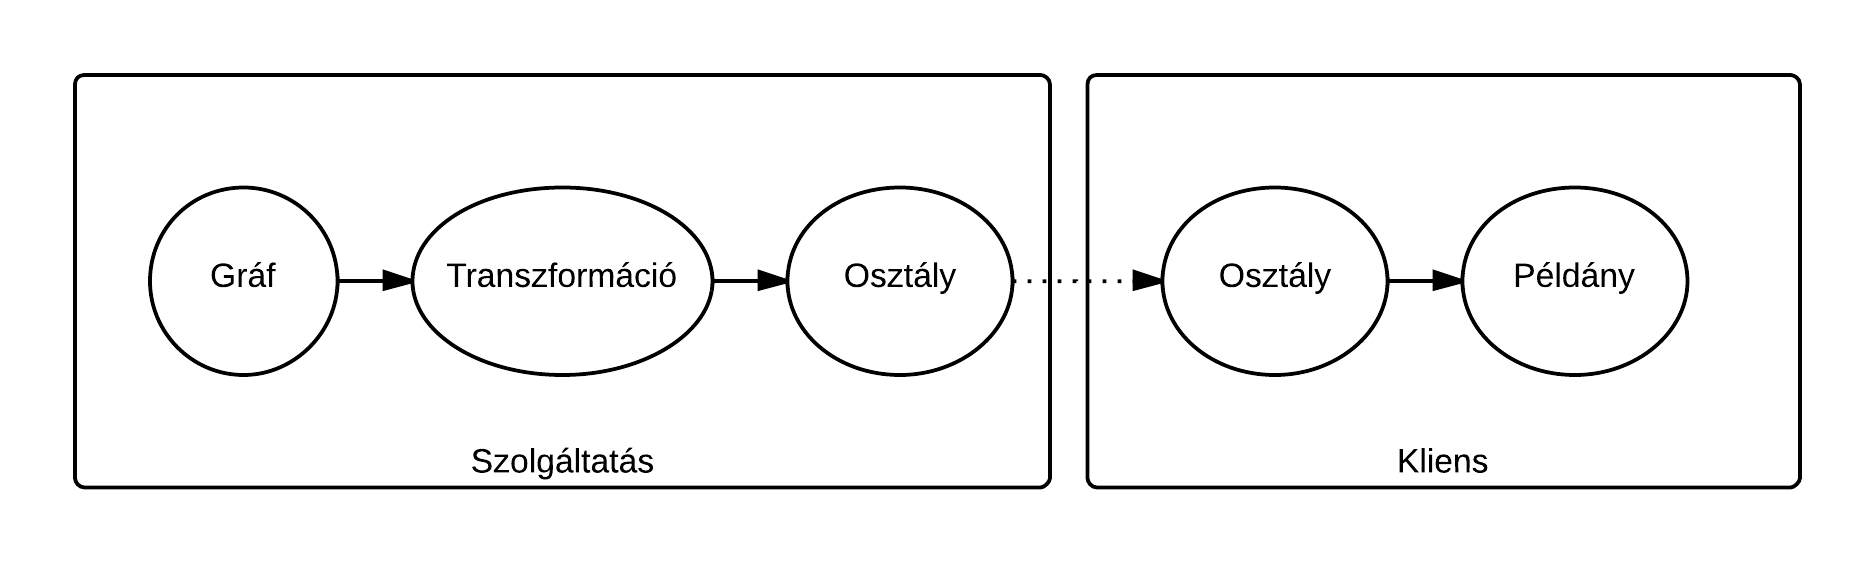
\includegraphics[width=\textwidth,height=\textheight,keepaspectratio]{figures/flow.png}\\
\caption{A szolgáltatás nagy vonalakban}
\label{fig:flow}
\end{figure}

A ~\ref{fig:flow} ábrán felhasználói szemszögből nézzük az alkalmazást, ezt el lehet érni akár szolgáltatásként a weben, vagy a kész munkára építve belső hálózaton saját magunk üzemeltethetünk egy példányt. A felhasználó a felületen létre tudja hozni a diagramot és a felületen létre tudja hozni a transzformációs logikát, a szerver majd értelmezi a kettőt és lefordítja kóddá, ami példáúl egy Javascript osztály lesz. A felhasználó majd ezt a komponenst a saját alkalmazásában szeretné használni és a szolgáltatás megfelelő API végpontján eléri ezt a kódot és a saját alkalmazásában példányosítja.



